\documentclass{report}[a4]
\usepackage{url}
\usepackage{epcc}
\usepackage{graphicx}
\usepackage[nottoc,numbib]{tocbibind}
\usepackage{listings, listings-rust}

\begin{document}
\title{Project Preparation Report}
\author{Jim Walker}
\date{\today}

\makeEPCCtitle

\thispagestyle{empty}

\pagebreak
\tableofcontents
\pagebreak

\chapter{Introduction}
This Project aims to examine the suitability of the new programming language Rust for use in high performance computing.

This Project Preparation report first provides a review of previous dissertations. It then presents the necessary background and literature for this project, High Performance Rust, and details a project proposal. A work plan for the project is sketched out, wherein we present chapter summaries and headings for the final dissertation alongside a Gantt chart. We identify risks and provide mitigations for them, before explaining our preliminary findings.
\chapter{Dissertation Review}
The two dissertations we have chosen to review are \textit{Assessing the Performance of Optimised Primality Tests}~\cite{Curry2016} by Cameron Curry, and \textit{Extending ePython to support ePython interpreting across multiple interconnected Epiphany processors}~\cite{Liang2017} by Dongyu Liang. Liang's \textit{Extending ePython} is focused on a programming language that is not typical in the High performance Computing (HPC) space, just our project will. Curry's \textit{Optimised Primality Tests} compared implementations of a core HPC function. Our project will compare our Rust implementation of some HPC code, with its original C implementation.
\section{Extending ePython}
Liang's dissertation chiefly reports on their efforts to extend ePython, a Python interpreter for the Epiphany processor, to `support parallel programming on multiple interconnected Epiphanies'~\cite{Liang2017}. An Epiphany processor has 16 cores, or e-cores, which makes it a useful platform for highly parallel codes. Liang first presents the technologies and paradigms which will they will use in their work. They go on to briefly describe the construction of their Epiphany cluster, before discussing at length their non trivial extension of ePython. Lastly, Liang closes with a results section which proves their achievements.

 \textit{Extending ePython} shows that Liang has made a useful contribution to high performance computing. Their technical achievement in extending ePython's parallelism to cover many nodes is notable, especially as Liang claims to make this change without compromising or altering the ePython programmer's interface. However, we can unfortunately only take their word for this, as their appendices only provide their  modified ePython. Liang does not include a listing of the form the original ePython would have taken.

 The introduction of \textit{Extending ePython} contains the assertion by Liang that the Epiphany processor `is  notoriously  difficult  to  program'~\cite{Liang2017}. Liang does not cite any sources for this claim, which is made somewhat dubious by the existence of a Python implementation precisely for the Epiphany processor.

 In the General Methodologies section (3.1.2) of the Construction (3.1), Liang discusses  `The principle of modifying ePython in the whole project is to make as few unnecessary adaptations as possible'~\cite{Liang2017}. Liang goes on to describe the methodologies used to develop their extensions, and clearly prioritises and justifies their design decisions. In this section Liang goes on to  discuss their implementation of host and device side routines. Whilst these details are useful to the reader in understanding how the e-cores communicate with each other, their inclusion in this section detracts from its clarity. This section could potentially be improved by moving the discussion of host and device side activities into their own part of the dissertation.

 Sections 3.2 and 3.3 of \textit{Extending ePython} contain a methodical presentation of Liang's extensions. Liang include all the detail necessary to understand what these extensions consist of, and provides useful figures to help the reader visualise some concepts. As these are very technical sections, it could perhaps be improved by the additions of some listings of pseudo-code to clarify the author's occasionally verbose description of a complex technology.

 We also question Liang's claims on the stability of their extension to ePython. Firstly, they do not precisely define what they mean by stability, whether they mean their system is numerically stable or if it simply does not crash. Secondly, Liang presents their code running on 32 cores across two nodes, presumably because they only had access to two nodes. Liang goes on to make the claim that their extension `could have become a cornerstone of the Supercomputer.io project'~\cite{Liang2017}, and saved it from its early end. The Supercomputer.io project was an attempt to collect multiple volunteer Epiphany based nodes across the internet to build an extremely large, extremely distributed cluster. Whilst Liang's extension to ePython would certainly have been a valuable contribution to the problems faced by Supercomputer.io, it is somewhat spurious for them to claim that their work could have been a `cornerstone' for this project. The high latency and large scale of the Supercomputer.io project is not really comparable to running a small cluster of two nodes, connected through a LAN.

 Liang closes with some benchmarks to display the performance of their ePython extensions. Liang's range of tests is comprehensive, and figure 4.5, showing the good parallel efficiency of the implementation is particularly interesting. We feel that figure 4.4, which shows the results of the strong scaling test on the cluster, could be improved by using more, larger problem sizes, and plotting them against speedup. This change would help make the test more indicative of future use cases, and make change in performance size and its affect on performance starker.

\section{Optimised Primality Tests}

In \textit{Optimised Primality Tests} Cameron Curry seeks to compare three different implementations of the Fermat Test, to assess which one PrimeGrid, a large distributed HPC project, should use. He argues that this is an important problem due to the extensive use of primes in computing, particularly cryptography. Curry also hopes to modify the Genefer implementation of the Fermat Test so that its residue calculation is consistent with other Fermat Test implementations.

Curry goes into great detail on the theoretical and practical background to his work. His frequent use of equations in section 2.1.4, `GFN Primes \& The Discrete Weighted Transform', show a firm grasp of the mathematical nature of his work, and how it is affected in hardware. Unfortunately Curry fails to emphasise how this background relates to his performance tests.  Whilst he does account for the `practicalities of digit representation in hardware', he does not make clear the effect this will have on his work, or how it is relevant to the specific performances of the implementations of the Fermat tests.

Curry goes on to describe his performance testing methodology, introducing the well accepted Roofline Model~\cite{williams2009, hennessy2011computer, asanovic2009view}, which he uses to estimate the peak performance of the processors he will run his test on. This valuable section is well documented and supported by useful figures and brief command extracts. Curry often both justifies his choices and details them with clarity, making his testing reproducible and understandable.

However, in Subsection 2.3.4, when Curry explains that his use of the Cray Performance Measurement and Analysis Tools (CrayPat) he does not justify his choice of tool. Curry uses CrayPat to inform the construction of his Roofline Model, and explains how CrayPat works in detail. He relays to the reader all  the commands which they should use to achieve the automatic profiling experiment to find the FLops/s and memory bandwidth of a given application, but those not state why CrayPat should be used rather than other alternatives.

Genefer is found to be the faster than both the LLR and OpenPFGW's Fermat Test implementations and Curry goes on to thoroughly investigate why that is. He uses tools such as the afore-mentioned CrayPat and the Roofline Model, to identify potential hardware bottlenecks and sources of software overhead. Curry even goes so far as to create a micro benchmark (page 28) to test an assumption about his tools, showing a rigorous approach to his experimentation.

Curry is motivated to modify Genefer's residue calculation due to its lack of consistency with OpenPFGW and LLR. This difference `is not an indication of incorrect results, it is simply a different representation of the least significant 64 bits'~\cite{Curry2016}. He goes on to document his modification of Genefer's residue calculation, first implementing it with the same library used by OpenPFGW and LLR and then developing his own implementation of it to maintain the application's portability.

The implementation of a consistent residue for Genefer is shown to be correct by retrieving the same outputs for a set of inputs. Curry is correct to call this feature only `potentially production ready for use', as he only shows us a few comparisons between calculations. To be sure that this implementation was ready would require much more testing of it than has been carried out here. Curry does not go into detail as to what would be needed for his implementation to become production ready, and only vaguely refers to carrying out `further correctness testing' in his conclusion.


\chapter{Background and Literature Review} %Why
Programming languages once offered few features, and were not very abstracted from the machine code. The first release of the Fortran compiler in 1957 only supported 32 statements~\cite{Backus:1957:FAC:1455567.1455599}. Although it provided the programmer with a minimal layer above the machine code which their programs would be translated to, it was quickly picked up by most of the programming community, because programs could be written faster, more easily, and were just as good as their machine code equivalent~\cite{metcalf2011seven}.

Programming languages have improved, and new languages are still released, generally with new features. The minority which was left writing hexadecimal has been replaced with a small group of people writing in C, C++ and Fortran. This is often down to the high level of performance which programmers can find in C, C++ or Fortran, evidenced by Turner's 2015 Archer white paper~\cite{Turner2015}, which found that Fortran continued to dominate in terms of per cent of total CPU cycles, as seen in Table~\ref{tab:langs}.
\begin{table}[h]
  \centering
  \label{tab:langs}
  \begin{tabular}{|c|c|c|c|c|}
    \hline
    & \textbf{HECToR Phase 2a} & \textbf{HECToR Phase 2b} & \textbf{HECToR Phase 3} & \textbf{Archer} \\
    \hline
    Fortran & 66.3\% & 65.2\% & 66.8\% & 69.3\% \\
    \hline
    C++ & 8.9\% & 2.7\% & 4.4\% & 7.4\% \\
    \hline
    C & 0.4\% & 3.6\% & 5.4\% & 6.3\% \\
    \hline
    Unidentified & 29.1\% &  30.0\% & 24.2\% & 19.4\% \\
    \hline
  \end{tabular}
  \caption{Breakdown of usage by programming language~\cite{Turner2015}}
\end{table}

Whilst Fortran and C or C++ are still being worked on and improved, they are unable to stray too far from their foundations, due to a mixture of cultural and technical reasons. This means these Fortran and C or C++ are unable to adopt all the new features of more recent programming languages.

One of those features is memory safety. In Figure~\ref{fig:mem}, we reproduce from the paper \textit{What can the Programming Language Rust do for Astrophysics}~\cite{blanco-cuaresma_bolmont_2016} by Blanci-Cuaresma and Bolmont, a diagram showing the kind of errors which can happen in a programming language in which memory safety is not guaranteed.
Errors a, b and c can occur in either sequential or parallel code whilst d can only occur in parallel code. The effect of these errors on programs can vary from crashing the program to corrupting the program's output, to nothing at all, depending on how well the programmer manages the error. It is important to note that these issues can be harder to debug in massively parallel applications, as tracing which process is writing to which memory location is harder.

\begin{figure}[h]
  \centering
  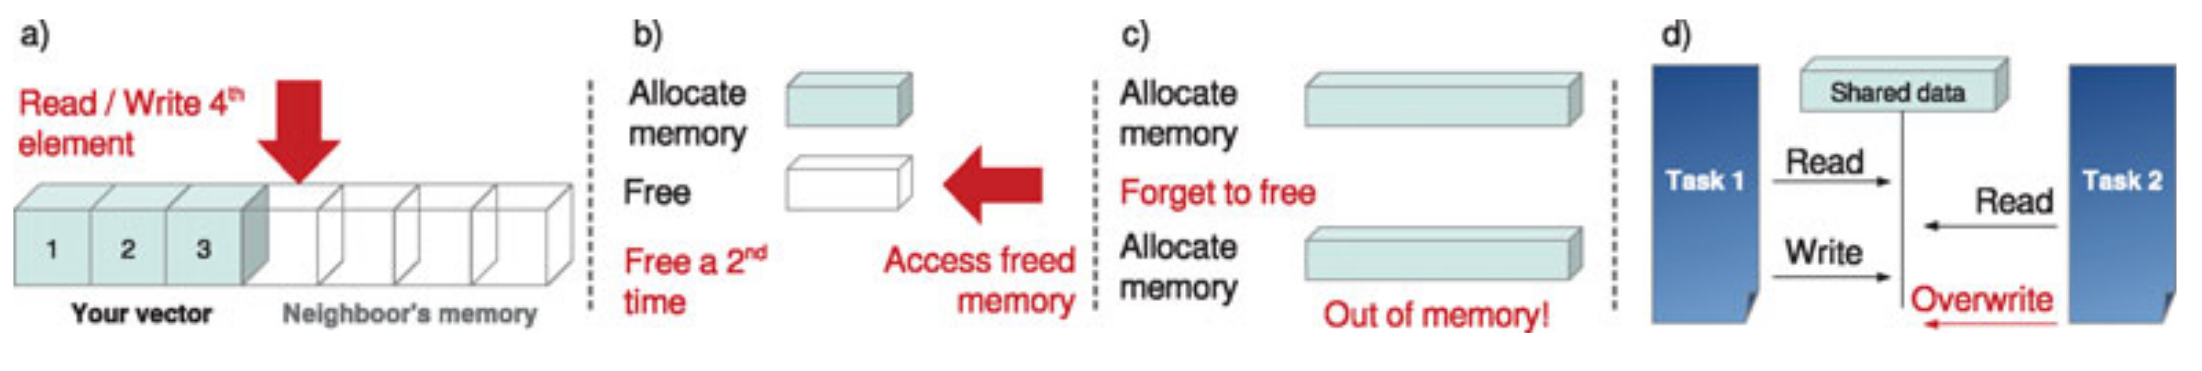
\includegraphics[width=\linewidth]{figures/memory-safety.png}
  \caption{`Potential Memory Safety Related Bugs'~\cite{blanco-cuaresma_bolmont_2016}. Reproduced with permission.}
  \label{fig:mem}
\end{figure}

No guarantee of memory safety has, in the past, been perceived by some programmers as the price to pay for granting the programmer fine grained memory control ~\cite{UCAM-CL-TR-798}. Fine grained memory control is part of what allows programmers to finely tune their codes to achieve the maximum performance from them. However, this means that the programmer must spend a significant portion of their time engaging in defensive programming, to ensure that memory safety bugs do not occur in their code.

A programming language's new features may make it an attractive contender for the HPC space, but it must also satisfy the criteria, e.g. fast parallelism, which C, C++ and Fortran already meet. Table~\ref{tab:langs} shows that new programming languages have failed to break into the HPC space, and meet these perceived criteria, for a variety of reasons. We will not attempt to formally define the criteria by which a programming language can become HPC appropriate in this report, but through examining some examples of languages which have so far failed to become widely used in HPC, we hope to begin work towards that criteria.

A 2008 paper found Java to be `acceptable when performing computational intensive tasks'~\cite{amedro}, but that it still faced a scaling problem for communication intensive tasks. It also found that whilst the Java Virtual Machine had improved considerably since early Java HPC efforts~\cite{philippsen2000javagrande}, that the performance of their benchmarks still varied greatly from one machine to another.

Other programming languages which aim directly for the HPC domain, like Chapel or UPC have so far failed to break into TIOBE's top 40 programming languages~\cite{TiobeMarch2019}. For a programming language to become widely used in HPC, one would expect it to be widely used outside of HPC, so that HPC users would benefit from the expertise a large group of general users could bring to a programming language.


The programming language Rust, first released in 2014, attempts to solve the problem of memory safety, without compromising the programmer's ability to control memory usage. `[P]ure Rust programs are guaranteed to be free of memory errors (dangling pointers, doublefrees) as well as data races'~\cite{Matsakis:2014}. Rust is not the first programming language to offer some of these features~\cite{Manson:2005:JMM:1047659.1040336, pygc, jones1996concurrent}. However, it is one of the first languages to contain all of these memory features at the same time, whilst simultaneously claiming to deliver performance comparable to C and Fortran. Rust also seems to be growing in popularity. Only five years after its initial release, it is ranked 35 in the TIOBE index, and its central GitHub repository has 34,826 stars and 5,596 forks~\cite{rustgit} only four years after its 1.0 release.

Some work has been done to investigate the applicability of Rust in scientific programming for bio-informatics~\cite{bioinformatics} and astro-physics~\cite{blanco-cuaresma_bolmont_2016}. Scientific kernels and applications such as the ones featured in these papers are common in HPC. The results of these investigations have been promising, and show that Rust is as fast, if not faster than implementations written in C or Fortran.

Rust's memory safety model also ensures that programmers do not need to make extra considerations to make their code memory safe. Consider the listing below where we add four to a value after checking it exists. In C we have to explicitly check if a value is null or not before proceeding with the operation. The programmer may forget to include this check, and potentially corrupt memory used by another part of the program, or even crash it.

\begin{lstlisting}[language=C]
// add_four.c
void add_four(int * foo){
    if(!foo){
        return;
    }
    *foo = *foo + 4;
}

void main(){
    int *a, var;
    var = 2;
    a = &var;
    add_four(a);
}

\end{lstlisting}
In comparison, the Rust version of this function needs no particular decoration to ensure that it is not carried out on an unexpected memory region. This is partly because Rust does not include null in the language. The closest equivalent that Rust has is the \texttt{Option<T>} type, like C++  \texttt{std::optional<T>}, which can either be \texttt{None} or \texttt{Some(value)}. This is very similar to Haskell's \texttt{Maybe} type. Rust forces the programmer to be mindful of when they might use a null pointer, and provides a simple, zero cost abstraction for dealing with it.
\begin{lstlisting}[language=Rust]
// add_four.rs
fn add_four(foo: &mut i32) {
    *foo = *foo + 4;
}

fn main() {
    let mut foo = 3;
    let bar = Some(&mut foo);
    bar.map(add_four);
}
\end{lstlisting}

Rust has many other features which are useful not just for general purpose programming, but HPC in particular. Rust's ownership memory model restricts values so that they can only ever by accessed through one owner, and must be explicitly borrowed to allow access. This leads to greater certainty about which process's functions are accessing which variables.

It is this memory model which allows parallel libraries like Rayon to exist. Rayon implements OpenMP style parallel loops, and because the rustc compiler is built on LLVM, it is able to efficiently vectorise code. Rust is certainly a strong contender for a HPC language, but it is as yet unproven. This dissertation project will aim to investigate how applicable Rust is to HPC. To achieve this aim, we will make use of mini-apps.

%Why mini apps
In high performance computing, `small self contained proxies for real applications' referred to as mini-apps~\cite{heroux2009improving}, are often used to test some particular configuration of a complex HPC stack~\cite{Mallinson:2014, Slaughter:2015, martineau2017arch}. As HPC systems and the applications which run on them are so complex, it is often difficult to accurately predict the performance of a HPC stack. This is a fundamental difficulty in comparing HPC configuration performances. Statistics comparing HPC clusters will often refer to a theoretical and a bench marked performance~\cite{top500}.

Mini-apps are intended to reflect the actual expected performance of a given class of HPC code on a given system, and therefore replicate the behaviour of real HPC kernels. There is a well documented precedent for using mini-apps to test different programming paradigms~\cite{Mallinson:2014, Slaughter:2015}. We will look to such approaches to inform our project.
%TODO expand this section

\chapter{Project Proposal} % What

Our research question follows: Can Rust be used to implement a high performance piece of software? We aim to answer this question by porting three existing HPC mini-apps or benchmarks into Rust, and then evaluating our implementation against the original. Our evaluation will inspect performance and scaling of the mini-apps, as well as programmablity. By programmability we mean we intend to judge our code base on how understandable it is by other, non Rust programmers, and how well it confirms to certain heuristics, i.e. loosely coupled and highly cohesive. We will also document the experience of learning Rust from a HPC programmer's perspective.

Suitable mini-app candidates will be selected using our own defined mini-app criteria, in an effort to ensure that ported mini apps are reflective of the real HPC programs written at the moment, make good use of Rust's unique features and are possible for one developer to implement in a three week sprint. For these reasons, our draft mini-app criteria are as follows:

\begin{itemize}
  \item The program's kernel (i.e. the part of the program where the majority of the processing is) should not be more than 1500 lines.
  \item The program should make extensive use of shared memory parallelism.
  \item The program should perform intense numerical operations on a data of at least a gigabyte.
  \item The original program should be written in C++, as we believe comparing Rust and C++ are most comparable, and C++ is of growing importance in HPC.
\end{itemize}

We hope that our criteria will then provide us with a shortlist of apps which we can then use to stress different aspects of Rust. For example, we hope to select one mini app which has a high CPU load, to test how efficiently Rust can process data, and another which has a high memory bandwidth requirement, to assess if Rust's memory model slows it down, or makes it difficult to program in. We present below our project goals.

\begin{enumerate}
  \item Find platform's theoretical hardware capabilities.
  \item Find three software artefacts that is representative of HPC use
  \item Port those software artefacts to Rust
  \item Assess how easily C or C++ developers can understand Software fragments
  \item Single Node Performance Tests
  \item Stretch goal - Multi node performance test
\end{enumerate}
\chapter{Work plan} % How
We have broken down this project into four main task groups. First, we will set up the project by defining and documenting our mini app criteria, which we will use to create a long list of mini apps. We will then select three mini apps to port from that long list. We will then benchmark the platform we will run our performance tests on, to ascertain its practical capability.

We will then build and benchmark the first of the mini apps which we are to port to Rust, before beginning development of the Rust version of the mini app. Throughout this development process we will take engineering notes to inform our later dissertation write up. The engineering notes will state what we were working on at given time, the challenges we faced, and how we overcame them. We will repeat this step for the other two benchmarks. Directly after finishing each benchmark we will carry out their performance tests, so that we can be reassured that no further development work will need to be done on that particular benchmark.

Finally, we will collate our engineering notes and carry out some small tests to assess the programmablity of our Rust mini-apps. We will then analyse all of the data we have collected, and finalise our dissertation, by collecting the project's existing documentation with our data analysis.

Below we present the planned structure for the final dissertation.
\begin{description}
  \item[Introduction]:
  \begin{itemize}
    \item Current state of Programming Languages in HPC.
    \item How are benchmarks/mini apps used in HPC.
  \end{itemize}
  \item[Background]:
    \begin{itemize}
    \item What features do programming languages need to be used in HPC?
    \item Why did D fail to replace C or C++ in HPC? What does this mean for Rust?
    \item What is Rust? What are its unique features of interest?
    \item How will our dissertation provide an indication of Rust's ability to succeed in HPC?
  \end{itemize}
  \item[Methods]:
\begin{itemize}
    \item Outline strict criteria used for selecting benchmarks.
    \item Describe software development process.
    \item Justify performance analysis processes.
  \end{itemize}
  \item[Implementation]:
  \begin{itemize}
    \item Overview of Software which we will port.
    \item Technical description of our implementation.
    \item Correctness testing.
  \end{itemize}
  \item[Performance Analysis]:
  \begin{itemize}
    \item How does performance compare to original app?
    \item How close do we get to hardware limit?
    \item Why does performance differ? (potentially go onto machine code analysis)
    \item How are both implementations affected by scaling?
  \end{itemize}
  \item[Programmablity]:
  \begin{itemize}
    \item Reflections on the experience of programming in Rust.
    \item Can other people understand it?
  \end{itemize}
  \item[Conclusion] :
  \begin{itemize}
    \item Summary of findings
    \item Further work
  \end{itemize}
\end{description}

\begin{figure}
  \centering
  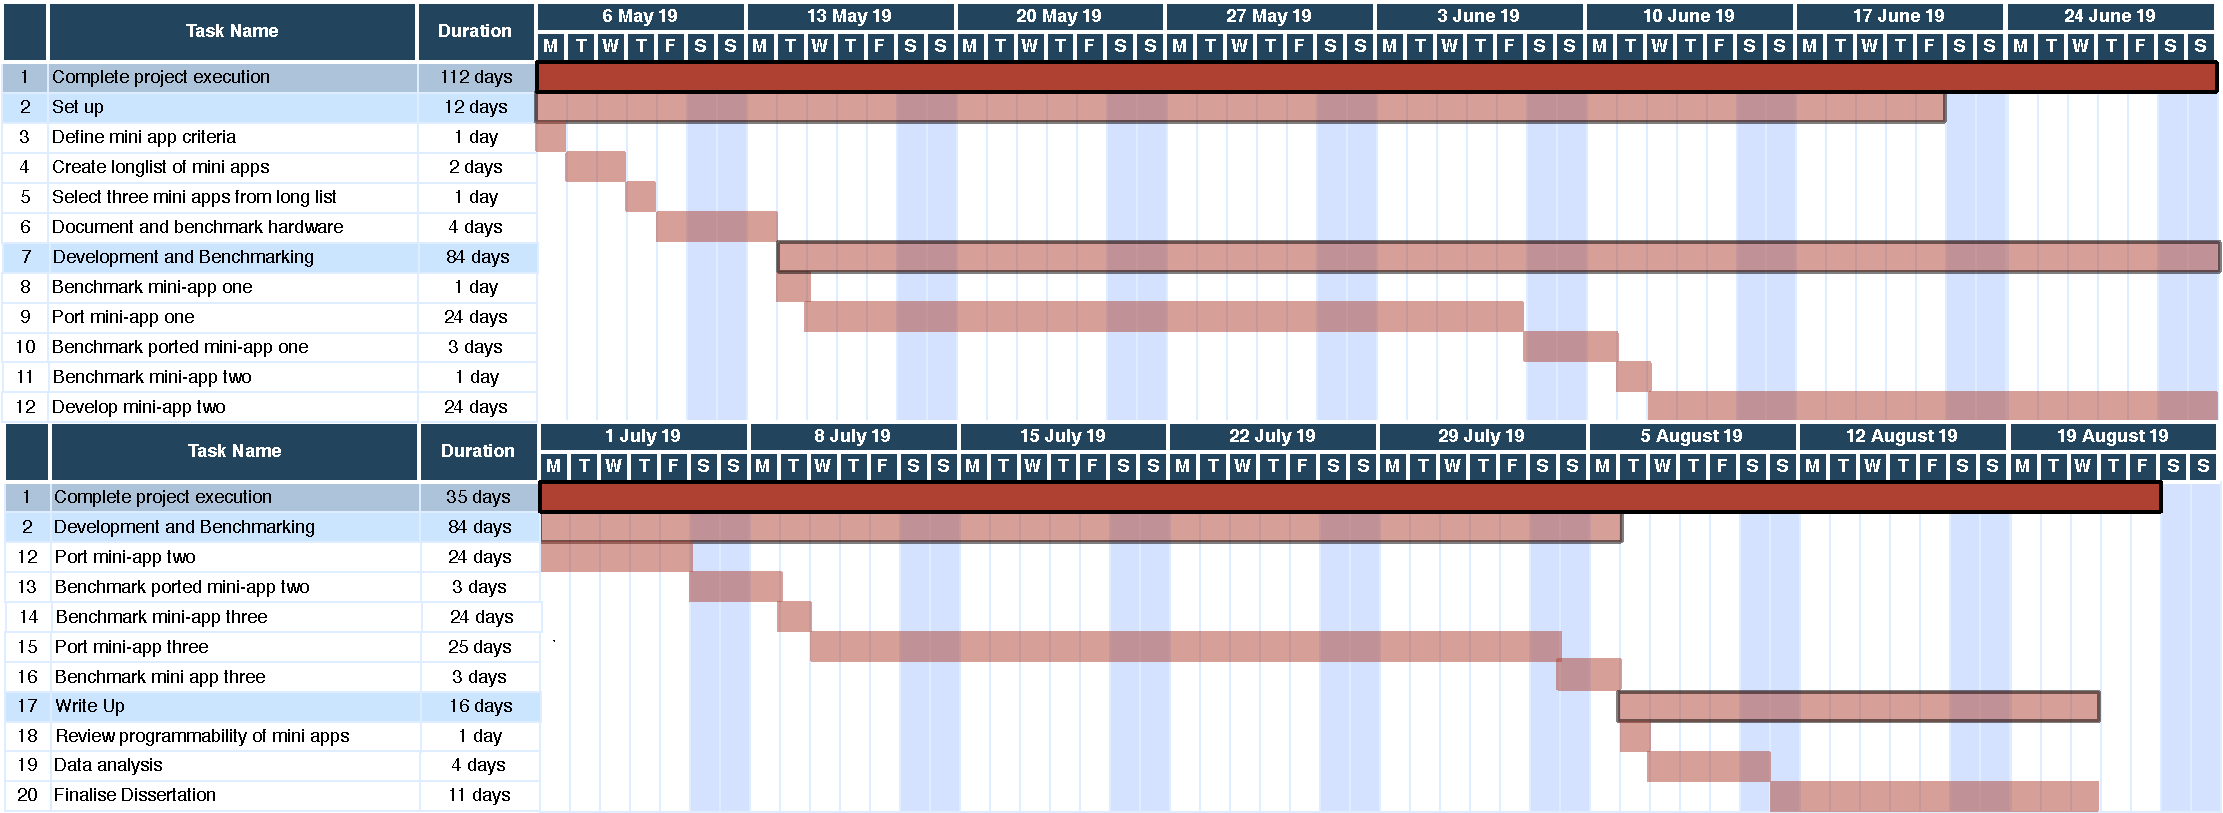
\includegraphics[angle=90, scale=0.6]{figures/dis_gantt.pdf}
  \caption{Project Gantt Chart}
  \label{}
\end{figure}

\chapter{Risk Analysis}
In planning our project, we have endeavoured to be aware of all risks to the project which are potential and plausible. We collected these risks through consultation with our dissertation supervisor and fellow students. We present these risks in our risk register (table~\ref{tab:risk}).

The most likely risk in the risk register is risk 3. It is normal for dissertation students to be given technical support in their dissertation projects by their dissertation supervisors and other EPCC with relevant domain knowledge. However, in our case the available technical support is likely to be more limited, as Rust is not a well known programming language amongst EPCC staff. Our mitigation for this risk is to rely upon the Rust community for issues which are particular to the Rust language. We do not expect the Rust community have a great deal of knowledge in the HPC space, but our expectation is that EPCC staff will be able to provide the necessary HPC expertise for us, whilst the Rust community provides guidance on the Rust language. It will fall to us to synthesise this knowledge where necessary, which is well within the objectives of this dissertation.

\section{Risk Register}
The risk register below is unordered. The listed risks were generated in consultation with Dissertation supervisors.

\begin{table}[h]
  \centering
  \begin{tabular}{c | p{4cm} c c p{4cm}}
  ID & Risk & Probability & Severity & Mitigation \\
    \hline
  1 &  Poor port selection & Medium & Medium & Confirm selection with advisers \\ \hline
  2 &  No knowledge of Rust amongst EPCC staff & High & Low & Rely on Rust community for language issues \\
    \hline
  3&  Rust Community has poor knowledge of HPC considerations & Medium & Low & No mitigation. We will have to take this risk and work around it. \\
    \hline
4 &    Run out of time for multiple node performance tests & Medium & Low & Jettison this goal. \\
\hline
5 & Run out of time to implement all benchmarks & Medium & Low & Drop benchmark. \\
    \end{tabular}
  \caption{Risk Register}
  \label{tab:risk}
\end{table}
\chapter{Preliminary Findings}
Thus far the work done in this project has been exploratory. We have implemented a simple program in C and in Rust, and compared performance. The program was a simple SAXPY (Single precision A$\times$X + Y) performed on a large array of random digits. We were not able to use this program to accurately compare the two programs, as we found Rust's aggressive \texttt{--release} optimisation (similar in intent to \texttt{-O3} found in C compilers) removed much of the processing done by the loop. This exercise illustrated to us some of the difficulties inherit in comparing two programming languages. Not only did we find proof that compiled programs are not wholly representative of their source code, we also found that `translating' a program from one language to another had its own pitfalls and considerations. We had to consider whether to use follow Rust idioms, like using iterators, or instead remaining more faithful to the C implementation and using a loop to increment a variable to access an array value. Ultimately, we have decided to write idiomatic, or Rustic Rust, unless there is more performant way to express the code.

As both C and Rust are Turing complete, Rust can express the same algorithms as C, and through the use of unsafe Rust, which allows the programmer to circumvent a lot of Rust's memory model, it is not especially difficult to write Rust that looks like C. If we write Rust to be like C, and especially if we write it in a way to avoid or minimise the features of Rust, then the comparison between implementations becomes less useful. However, we feel it is fair to deviate from idiomatic Rust where there are noticeable performance benefits and that deviation is minimal, due to the great emphasis HPC programmers place on performance.

We have installed Rust on Cirrus and compiled and run the simple SAXPY program mentioned above. We have also found the Rust package management system, cargo, to work with no required set up. This package system is similar to python's pip or Node JS's npm and does not require administrator privileges. We believe this will be useful to HPC developers, as Rust follows a `batteries not included' philosophy, requiring users to download and install packages for common utilities like random number generation. HPC systems often restrict administrator privileges, so it is important developers can access libraries without it. Alongside our simple programs, we have compiled some complex Rust programs with higher number of dependencies~\cite{Bat,Exa} on Cirrus and found them to operate as normal. However, we have yet to experiment with any highly parallel Rust codes on Cirrus yet.

We have begun research into Rust's memory model through some practical exercises found on the Rust by Example website~\cite{rustbyexample}. Initial contact with the rust community has been made through the \#rust-beginners IRC channel on \url{irc.mozilla.org}, and we have found them helpful in troubleshooting some of our issues. Rust's HPC relevant features have also been explored, and we have found the Rayon library which uses a potential parallelism approach to multi-threading. That is, given the statement below, code may or may not run in parallel.

\begin{lstlisting}[language=Rust]
join(|| do_something(), || do_something_else())
\end{lstlisting}

In Rayon, `the decision of whether or not to use parallel threads is made dynamically, based on whether idle cores are available'~\cite{rayon}. Removing the ability to make workload distribution decisions from the programmer can run counter to traditional HPC philosophies of fine grained control, but as Rayon promises data race freedom, it might be a price worth paying.

We have also made steps towards formalising the desired qualities of any potential new HPC language.

\begin{itemize}
  \item It must be widely used outside of the HPC community, so that there is a large pool of people who can use it, and so that the language can be actively improved by people who's main concern is not HPC.
  \item It must be capable of instruction level parallelism
  \item It must be capable of shared and distributed memory parallelism.
  \item It must be compatible with MPI.
  \item It must provide low level memory management.
\end{itemize}

We have included the justification for many of the items in this list in our background section, but we have added compatibility with MPI purely because such a high number of HPC codes use them.

Our research into mini-apps has already found some potential candidates, including Babel Stream, a memory bandwidth benchmark~\cite{raman2017improving}. We have also found a collection of mini-apps from the UK mini-app consortium~\cite{MAC}, and are likely to select one of their pieces of software too.

\chapter{Conclusion}
We have presented the work we have done in preparation for our dissertation. Whilst Rust appears to have many of the attributes one might associate with a HPC language, its actual ability to perform in HPC tasks and at scale are yet to be proven in a through investigation. This project aims to start that investigation. We have considered the risks to our project, and planned accordingly.

\bibliographystyle{plain}
\bibliography{bib}
\end{document}
